\section{Sicherheitsvollständige Testsuite (\emph{safety-complete Test Suite})}
\begin{frame}
\frametitle{Safety-related Output Abstraction}
\begin{itemize}
  \item Reaktion des Systems wird durch DFSM-Ausgabe modelliert
  \item Idee: Falsche Ausgabe muss nicht sicherheitsrelevant sein
  \item Sicherheitskritische Reaktionen definieren
  \item Nicht-sicherheitskritische Reaktionen zusammenfassen
\end{itemize}
\end{frame}

\begin{frame}
\frametitle{Safety-related Output Abstraction}
\begin{itemize}
  \item \emph{safety-related output abstraction}: $\leq_s \subseteq \Sigma_O \times \Sigma_O$
  \item $\leq_s$ sei reflexiv, transitiv.
  \item z.B: Warnsystem bei einer stationären Überwachung im Krankenhaus\\
  $$\Sigma_O = \{\texttt{OK}, \texttt{Tech-Warnung}, \texttt{Med-Warnung}, \texttt{Notfall}\}$$
  $$\texttt{OK} \leq_s \texttt{Tech-Warnung} \leq_s \texttt{Med-Warnung} \leq_s \texttt{Notfall}$$
\end{itemize}
\end{frame}

\begin{frame}
  \frametitle{Sicherheitsäquivalenz}
  \begin{itemize}
    \item s-äquivalent: $y_1 \sim_s y_2 \equiv y_1 \leq_s y_2$ und $y_2 \leq_s y_1$
    \item Zwei Ausgabesequenzen: $$\omega \sim_s \pi \equiv (\#\omega = \#\pi \wedge \forall i \in \{1,\ldots,\#\omega\} : \omega(i) \sim_s \pi(i))$$ 
    \item Zwei Zustände: $$q \overset{\overline{x}}{\sim_s} q' \equiv \lambda(q,\overline{x}) \sim_s \lambda(q', \overline{x})$$
    $$q \sim_s q' \equiv q \overset{\Sigma_I^*}{\sim_s} q'$$
    \item Zwei Systeme sind s-äquivalent gdw. ihre Anfangszustände s-äquivalent sind.
  \end{itemize}
  \end{frame}

\begin{frame}
\frametitle{Safety-Complete Test Suite}
Eine Test Suite $TS$ wird \emph{safety complete} genannt, gdw. für jedes SUT~$M'$ der Fehlerdomain gilt:
\begin{itemize}
  \item Soundness: $M$ und $M'$ sind I/O-äquivalent zueinander $\Rightarrow$ $M'$ besteht die Teset Suite ($M'~ \underline{pass}~ TS$)
  \item safety-Exhaustiveness: Für alle $M'$ aus der Fehlerdomain gilt: $M' \not \sim_s M \Rightarrow M'~ \underline{fail}~ TS$
\end{itemize}
\end{frame}

\begin{frame}
\frametitle{Beispiel}
\begin{columns}[T] % align columns

\begin{column}{.50\textwidth}
\textbf{M}
\includegraphics[width=\textwidth]{images/fsm-example01}
\end{column}%

\begin{column}{.50\textwidth}
\textbf{Safety Abstraktion von M}\\
\begin{itemize}
  \item $0 \sim_s 1 \leq_s 2$
  \item Ausgaben $0,1$  $\rightarrow Y$
  \item Ausgabe $2$ bleibt unverändert
\end{itemize}
\end{column}%
\end{columns}
\end{frame}



\begin{frame}
\frametitle{Beispiel}
\begin{columns}[T] % align columns

\begin{column}{.50\textwidth}
\textbf{M}
\includegraphics[width=\textwidth]{images/fsm-example01}
\end{column}%

\begin{column}{.50\textwidth}
\textbf{Sicherheitsabstraktion von M}
\only<1>{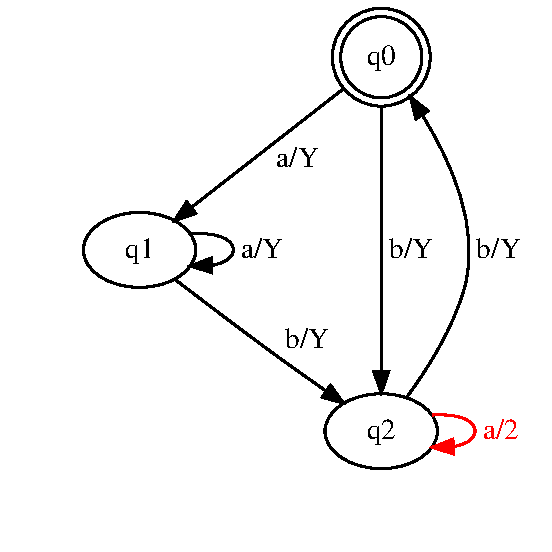
\includegraphics[width=\textwidth]{images/fsm-example01_abs}}%
\only<2->{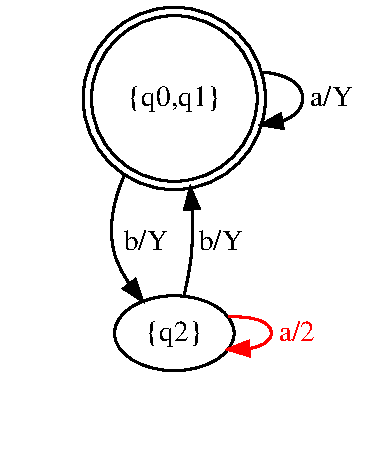
\includegraphics[width=0.8\textwidth]{images/fsm-example01_abs_min}}%
\end{column}%
\end{columns}
\end{frame}

\begin{frame}

\frametitle{Safety-H Methode}
\begin{center}
  \scriptsize
\emph{Huang, W., Özoguz, S. \& Peleska, J. Software Qual J (2018)}\\
\end{center}
\normalsize
$(\alpha, \beta)$-Liste stammt aus den gleichen Mengen wie bei der $H$-Methode
\begin{itemize}
    \item $A=V\times V$
    \item $B=V\times (V.\bigcup\limits_{i=1}^{m-n+1}.\Sigma_I^i)$
    \item $C=\{(\alpha,\beta)|\alpha,\beta\in V.\bigcup\limits_{i=1}^{m-n+1}.\Sigma_I^i, \alpha \in \text{Pref}(\beta)\}$
  \end{itemize}

\begin{columns}[T] % align columns
\begin{column}{.50\textwidth}
\pause
\begin{itemize}
  \item<2-> $(\alpha, \beta) \in A, \delta(q_0,\alpha) \not \sim \delta(q_0, \beta)$
  \item<3-> $(\alpha, \beta) \in B, \delta(q_0,\alpha) \not \sim_s \delta(q_0, \beta)$
  \item<3-> $(\alpha, \beta) \in C, \delta(q_0,\alpha) \not \sim_s \delta(q_0, \beta)$
\end{itemize}
  \end{column}%
  \begin{column}{.60\textwidth}

  \begin{itemize}
  \item[]<2-> \textcolor{blue}{\underline{\textcolor{black}{Wie in $H$-Methode}}}
  \item[]<3-> \textcolor{red}{\underline{\textcolor{black}{Weniger Zustände unterscheidbar}}}
\end{itemize}
\end{column}
\end{columns}

\end{frame}

\begin{frame}
\frametitle{Safety-H Methode}
\begin{itemize}
  \item Verallgemeinerung der $H$-Methode
  \item Je weniger Zustände die Abstraktionsmaschine hat, desto weniger Testfälle werden erzeugt
\end{itemize}
\end{frame}